\documentclass{article}
\usepackage[utf8]{inputenc} % Suporte para UTF-8
\usepackage{spverbatim} % Para incluir código com quebras de linha
\usepackage{graphicx} % Para incluir imagens
\usepackage{float} % Para manter a imagem fixa e texto após ela (driblar a otimização do latex) [H]
\usepackage{caption} % Para adicionar legendas fora do ambiente figure
\title{Coding the main tex (Rstudio, Excel - in progress)} % Define o título do documento
\author{Thiago  Vinicius Gomiero} % Define o autor do documento
\date{February 2024} % Define a data que aparece no documento

\begin{document}

\maketitle % Este comando cria o título do documento, autor e data previamente definidos
\section{Explanation of the codes used in RStudio and Excel}
\subsection{Rsutio code}

\begin{spverbatim}
# Loads the xtable library, which provides functions for exporting tables to LaTeX or HTML
library(xtable)

# Creates a vector of cells with numeric values
cells <- c(39, 331, 326, 26, 0, 772, 40, 591, 1010, 170, 4, 1815, 19, 312, 1144, 488, 18, 1981, 5, 100, 479, 290, 23, 897, 0, 17, 120, 153, 27, 317, 103, 1351, 3079, 1127, 72, 5732)

# Creates a vector of column names
cnames<-c("33-35", "36-38", "39-41", "42-44", "45-over", "Row totals")

# Creates a vector of line names
rnames<-c("64-65", "66-67", "68-69", "70-71", "72-73", "Column totals")

# Creates a matrix from the vector of cells, with 6 rows and 6 columns, and assigns the names of the rows and columns
matrixdata<-matrix(cells, nrow=6, ncol=6, byrow=TRUE, dimnames=list(rnames,cnames))

matrixdata #Display the matrix

# Print the matrix as a LaTeX table using the xtable function
print(xtable(matrixdata), type="latex")
-> The final result of this is:
\end{spverbatim}
\begin{center}
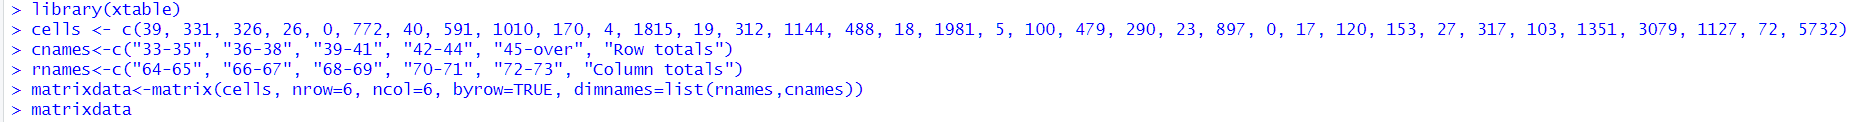
\includegraphics[width=\linewidth]{imagesfolder/image.png}
\label{fig:enter-label1}

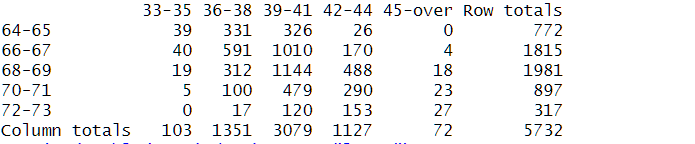
\includegraphics[width=\linewidth]{imagesfolder/image3.png}
\label{fig:enter-label2}

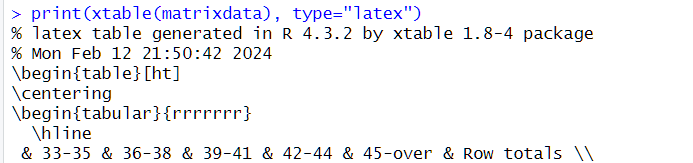
\includegraphics[width=\linewidth]{imagesfolder/image4.png}
\label{fig:enter-label3}

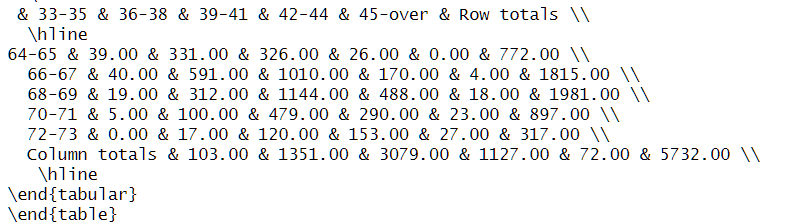
\includegraphics[width=\linewidth]{imagesfolder/image5.png}
\label{fig:enter-label4}
\end{center}
\begin{spverbatim}
Where I simply copy the code and paste in LaTex:
\end{spverbatim}
\begin{center}
   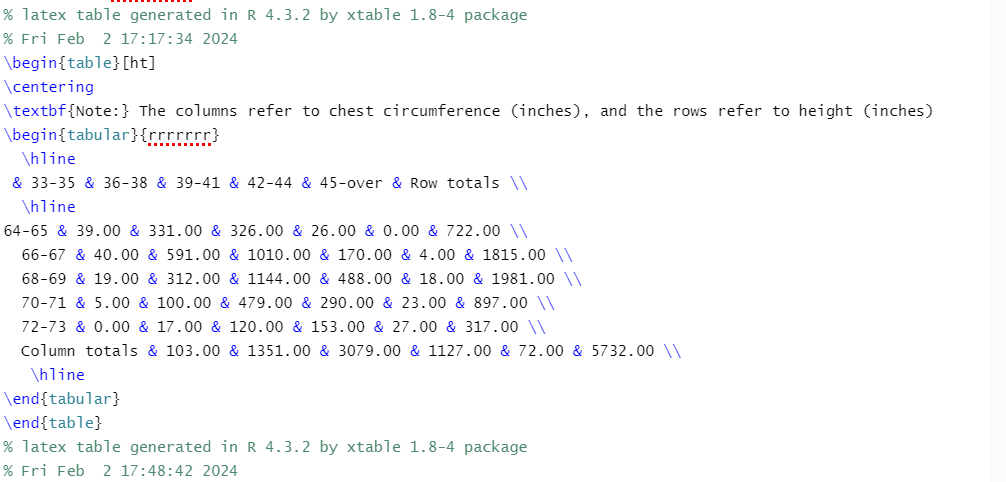
\includegraphics[width=\linewidth]{imagesfolder/image6.png}
\label{fig:enter-label5} 
\end{center}

The use of fig:enter-label is for future reference: reference each image individually elsewhere in your document using \verb|\ref{fig:label1}, \ref{fig:label2}|, etc.

\subsection{Rsutudio code}
The following code is akin to the first one. In fact, only the content changes, but the structure and the results remain unchanged.
\begin{spverbatim}

# Creates a second vector of cells with numeric values
cells2<-c(66.31, 66.84, 67.89, 69.16, 70.53, 38.41, 39.19, 40.26, 40.76, 41.80)

# Creates a vector of line names
rnames2<-c("mean of height given chest-inches ", "mean of chest given height-inches")

# Creates a second matrix from the cell vector, with 2 rows and 5 columns, and assigns the row names
matrixresum<-matrix(cells2, nrow=2, ncol=5, byrow=TRUE, dimnames=list(rnames2))

matrixresum #Display the matrix

# Print the matrix as a LaTeX table using the xtable function
print(xtable(matrixresum), type="latex")
\end{spverbatim}

\subsection{Rstudio code}
\begin{spverbatim}
# Install the package 'readr', which contains functions for reading tabulated data.
install.packages("readr") 

# Load the package "readr" for use
library(readr)

# Defines the path to the file CSV that needs to be read
caminho_arquivo <- "C:\\Users\\gomie\\Downloads\\datalife.csv"

# Read the CSV file and save its content in the variable "dados".
dados <- read_csv(caminho_arquivo)

# Exhibit the first 6 lines of the dataset.
head(dados)
\end{spverbatim}


The result of these first lines above is this in the Rstudio:
\begin{figure}[H]
    \centering
    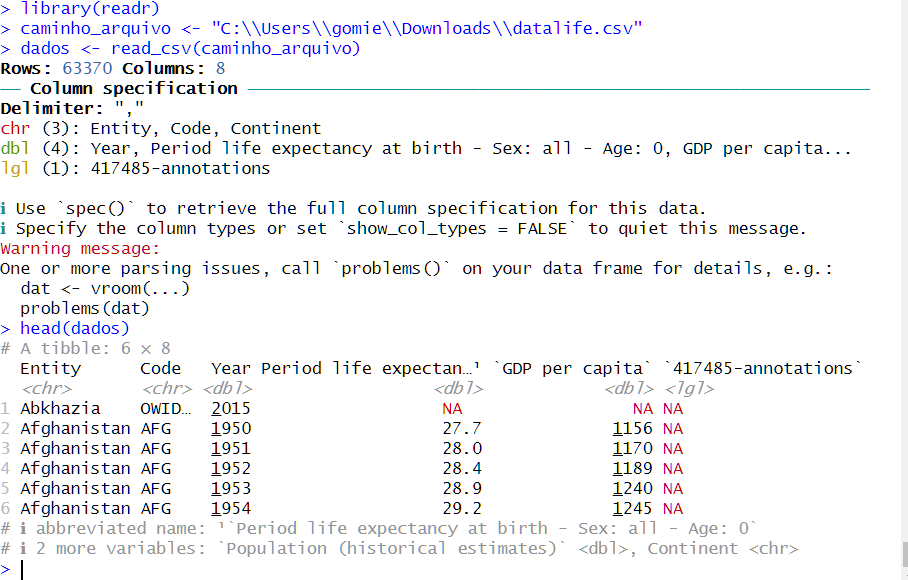
\includegraphics[width=1\linewidth]{imagesfolder/image11.png}
\end{figure}


\begin{spverbatim}
# Finds unique values in the 'Entity' column of the dataset and stores them in the 'entities' variable.
\end{spverbatim}
\begin{verbatim}
entidades <- unique(dados$Entity)
\end{verbatim}
\begin{spverbatim}
# Prints the unique values found.
print(entidades) 

# Creates a subset of the data where the entity is 'Brazil' and stores it in the variable 'dados_brazil'.
dados_brazil <- subset(dados, Entity == "Brazil")

#Prints the data subset for 'Brazil'.
print(dados_brazil)
\end{spverbatim}

The result of these first lines above is this in the Rstudio (continues until [327]:
\begin{figure}[H]
    \centering
    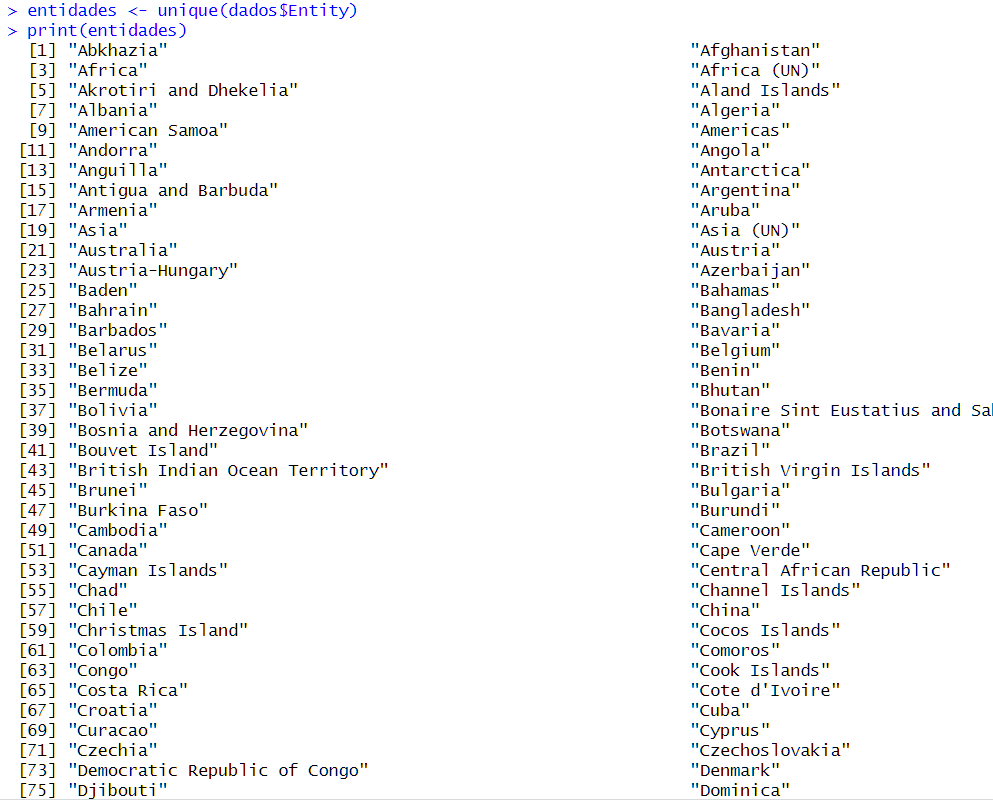
\includegraphics[width=1\linewidth]{imagesfolder/image12.png}
\end{figure}
and:
\begin{figure}[H]
    \centering
    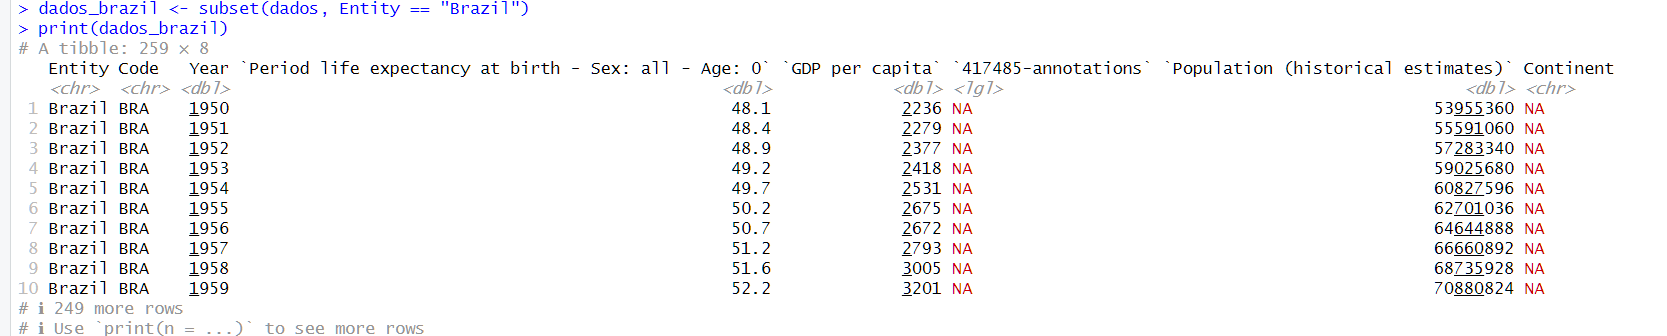
\includegraphics[width=1\linewidth]{imagesfolder/image13.png}
\end{figure}

\begin{spverbatim}
# Creates a subset of the data for 'Brazil' where the year is between 1950 and 2010.
dados_brazil_1950_2010 <- subset(dados_brazil, Year >= 1950 & Year <= 2010)

# Prints the subset of data for 'Brazil' between 1950 and 2010.
print(dados_brazil_1950_2010)

# Prints the first 100 rows of the data subset for 'Brazil' between 1950 and 2010
print(dados_brazil_1950_2010, n = 100)
\end{spverbatim}

The result of these first lines above is this in the Rstudio (the last one continues until 2010) :
\begin{figure}[H]
    \centering
    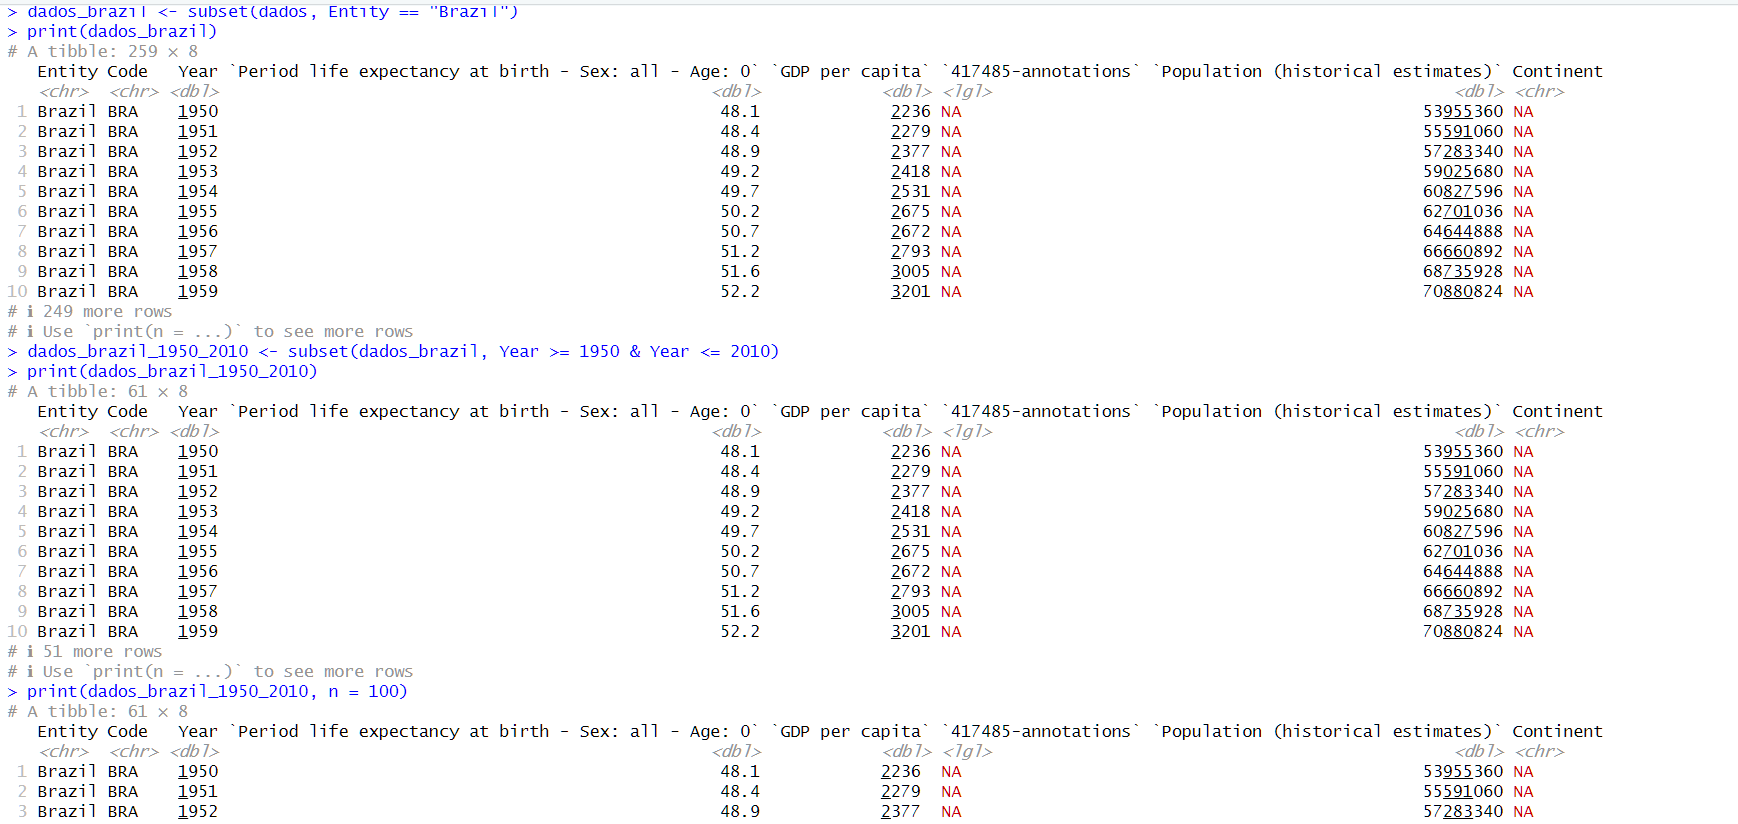
\includegraphics[width=1\linewidth]{imagesfolder/image14.png}
\end{figure}

\begin{spverbatim}

# Calculates the correlation between 'GDP per capita' and 'Period life expectancy at birth - Sex: all - Age: 0' for 'Brazil' between 1950 and 2010.
# "complete.obs": excludes pairs of observations with the NA value in the corresponding variable. This means that observations must be complete for each variable analyzed.
correlacao <- cor(dados_brazil_1950_2010$`GDP per capita`, dados_brazil_1950_2010$`Period life expectancy at birth - Sex: all - Age: 0`, use="complete.obs")

# Prints the calculated correlation value.
print(correlacao)
\end{spverbatim}

\begin{verbatim}
# Prints a statistical summary for 'GDP per capita' for 'Brazil' between 1950 and 2010.
print(summary(dados_brazil_1950_2010$`GDP per capita`))
\end{verbatim}
The result of these first lines above is this in the Rstudio:
\begin{figure}[H]
    \centering
    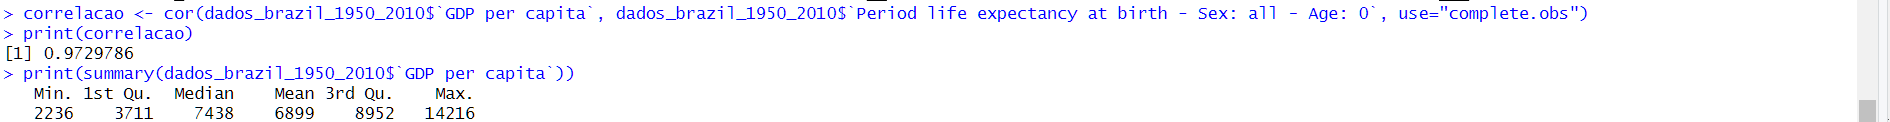
\includegraphics[width=1\linewidth]{imagesfolder/image15.png}
\end{figure}

\begin{spverbatim}

# Starts recording a graphic to a PNG file.
# The first argument of png, in this case "meu_grafico.png" indicates the name of the file that will be saved.
png("meu_grafico.png", width = 800, height = 600)

# Creates a scatterplot of 'GDP per capita' versus 'Period life expectancy at birth - Sex: all - Age: 0' for 'Brazil' between 1950 and 2010.
plot(dados_brazil_1950_2010$`Period life expectancy at birth - Sex: all - Age: 0`, dados_brazil_1950_2010$`GDP per capita`,
     xlab = "Life expectancy",
     ylab = "GDP per capita",
     main = "GDP per Capita vs Life expectancy at birth in Brazil (1950-2010)")

# Closes the graphics device and saves the PNG file.
dev.off()

#The value 2 that is returned after calling dev.off() indicates that the RStudioGD graphics device is now active again. This means that any subsequent graphs you create will be displayed in RStudio's plot window, rather than being routed to a PNG file.
#To know where the file will be saved, you need to check the current working folder. It is possible to find out which one it is using the getwd() command.
If you want to change the current working folder, you can do this with the setwd() function.
Example: setwd("C:\Users\gomie\OneDrive\estat"). Remember to replace the slash \ with 2 single slashes \\ or one backslash.
To manually add a specific save location, it would be for example: png("C:/Users/gomie/OneDrive/estat/meu_grafico.png", width = 800, height = 600)
\end{spverbatim}
The result of these first lines above is this in the Rstudio:
\begin{figure}[H]
    \centering
    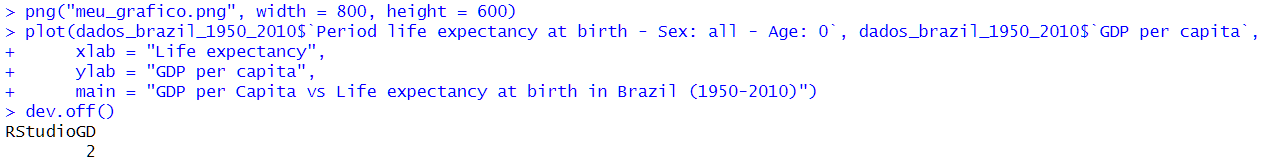
\includegraphics[width=1\linewidth]{imagesfolder/image16.png}
\end{figure}
\begin{figure}[H]
    \centering
    
\includegraphics[width=1\linewidth]{imagesfolder/image17.png}
\end{figure}
\begin{figure}[H]
    \centering
    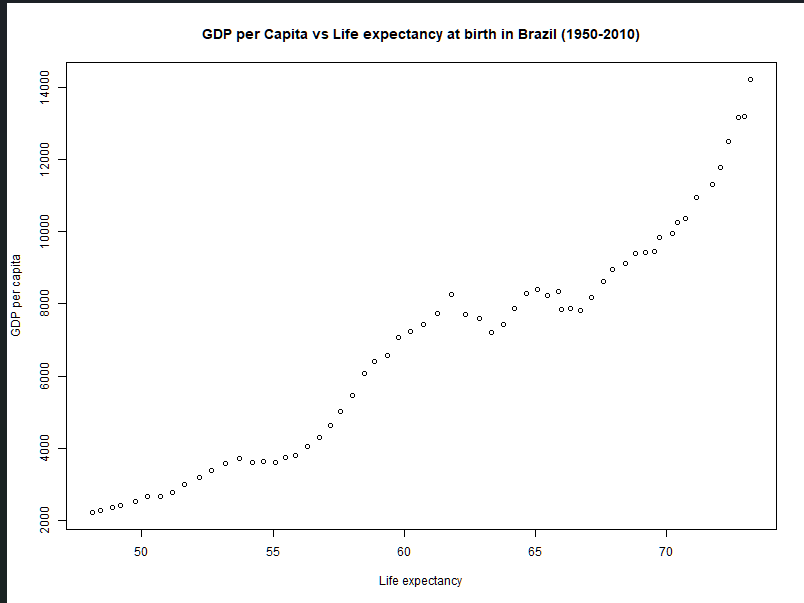
\includegraphics[width=1\linewidth]{imagesfolder/image18.png}
\end{figure}

\begin{spverbatim}
# Install the 'xtable' package, which provides functions for exporting tables to LaTeX or HTML.
install.packages("xtable")

# Load the 'xtable' package for use.
library(xtable)

# Creates a subset of the data for 'Brazil' between 1950 and 2010 with the columns 'Year', 'Period life expectancy at birth - Sex: all - Age: 0', and 'GDP per capita'.
# In R, the comma is used to separate dimensions in an array or a data frame. The part before the comma refers to the rows and the part after the comma refers to the columns.
dados_brazil_1950_2010[, c("Year", "Period life expectancy at birth - Sex: all - Age: 0", "GDP per capita")], the part before the comma is empty, which means selecting all lines in the table of data. The part after the comma is a vector of column names, which means selecting only those specific columns.
dados_tabela <- dados_brazil_1950_2010[, c("Year", "Period life expectancy at birth - Sex: all - Age: 0", "GDP per capita")]

# Rename the data subset columns.
#In R, the colnames() function is used to get or set the names of the columns of an object, such as a data frame. In the code, colnames(table_data) <- c("Year", "Life Expectancy", "GDP per Capita") is redefining the names of the columns of the table_data data frame.
colnames(dados_tabela) <- c("Ano", "Expectativa de Vida", "PIB per Capita"

# Converts the subset of data into a LaTeX table.
tabela_latex <- xtable(dados_tabela)

# Prints the LaTeX table in a file called 'table.tex'.
#type="latex": This specifies to print the object as LaTeX code.
file = "table.tex": This specifies the name of the file where the LaTeX code will be saved. In this case, the code will be saved in a file called “table.tex”. tabular.environment = "longtable": This specifies the LaTeX longtable environment for the table. The longtable environment allows tables to span multiple pages, which is useful for very long tables. floating = FALSE: In LaTeX, tables are typically placed in a floating environment, which means that LaTeX can move the table to a different location to better fit the page. If floating = FALSE, the table will be placed exactly where it appears in the code, and will not be moved.
print(tabela_latex, type = "latex", file = "tabela.tex", tabular.environment = "longtable", floating = FALSE)
\end{spverbatim}
The result of these first lines above is this in the Rstudio:
\begin{figure}[H]
    \centering
    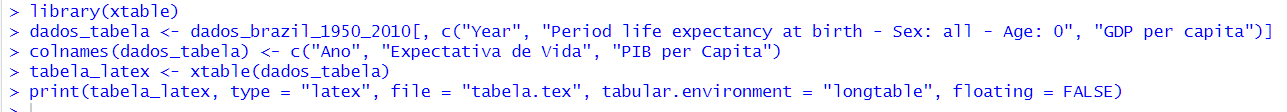
\includegraphics[width=1\linewidth]{imagesfolder/image19.png}
\end{figure}

\begin{figure}[H]
    \centering
    
\includegraphics[width=1\linewidth]{imagesfolder/image20.png}
\end{figure}
\begin{spverbatim}
# To save the file in a specific location, include the full file path in the file argument. On Windows, use double slashes (\\) or backslashes (/).
print(tabela_latex, type = "latex", file = "C:/Users/gomie/OneDrive/estat/tabela.tex", tabular.environment = "longtable", floating = FALSE)

# Install the 'knitr' package, which provides functions for dynamic reporting.
install.packages("knitr")

# Carrega o pacote 'knitr' para uso.
library(knitr)

# Calculates the correlation between 'GDP per capita' and 'Period life expectancy at birth - Sex: all - Age: 0' for 'Brazil' between 1950 and 2010.
correlacao <- cor(dados_brazil_1950_2010$`GDP per capita`, dados_brazil_1950_2010$`Period life expectancy at birth - Sex: all - Age: 0`, use="complete.obs")

# The sprintf function is used to format a string. It replaces each format specifier (%f) in the string with the value of the corresponding variable (in this case, 'correlation').
texto_latex <- sprintf("The correlation between GDP per capita and life expectancy at birth in Brazil (1950-2010) is %f.", correlacao)

# The writeLines() function is used to write text to a file. writeLines(texto_latex, con = "correlacao.tex") is writing the contents of text_latex to a file called “correlacao.tex”. The con argument specifies the file name.
writeLines(texto_latex, con = "correlacao.tex")

The result of these first lines above is this in the Rstudio:
\end{spverbatim}
\begin{figure}[H]
    \centering
    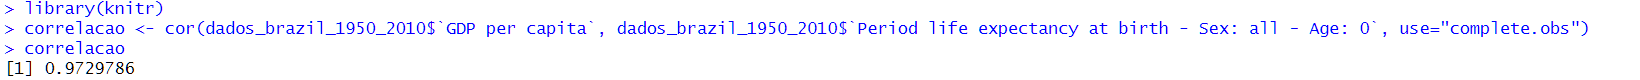
\includegraphics[width=1\linewidth]{imagesfolder/image23.png}
\end{figure}
\begin{figure}[H]
    \centering
    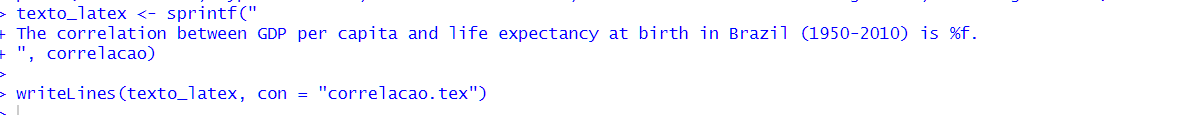
\includegraphics[width=1\linewidth]{imagesfolder/image21.png}
\end{figure}
\begin{figure}[H]
    \centering
    
\includegraphics[width=1\linewidth]{imagesfolder/image22.png}
\end{figure}

\subsection{Rstudio code}
\begin{spverbatim}

# Creates a matrix with the data
#This part of the code creates an array called data with 3 columns. Numbers are entered into the matrix row by row (byrow = TRUE).
data <- matrix(c(
  .28, .03, .0,
  .08, .15, .03,
  .04, .06, .06,
  0, .06, .15,
  0, 0, .03,
  0, 0, .03,
  .40, .30, .30,
  1.4, 2.5, 3.9,
  .44, .85, 1.09
), ncol = 3, byrow = TRUE)

# Assign names to columns and rows
colnames(data) <- c('20000', '30000', '40000')
rownames(data) <- c('1000', '2000', '3000', '4000', '5000','6000', 'Marginal Probability', 'Mean(Y|X)','Var(Y|X)')

# Converts the matrix to a table
table <- as.table(data)

# Print the table
print(table)
\end{spverbatim}
The result of these first lines above is this in the Rstudio:
\begin{figure}[H]
    \centering
    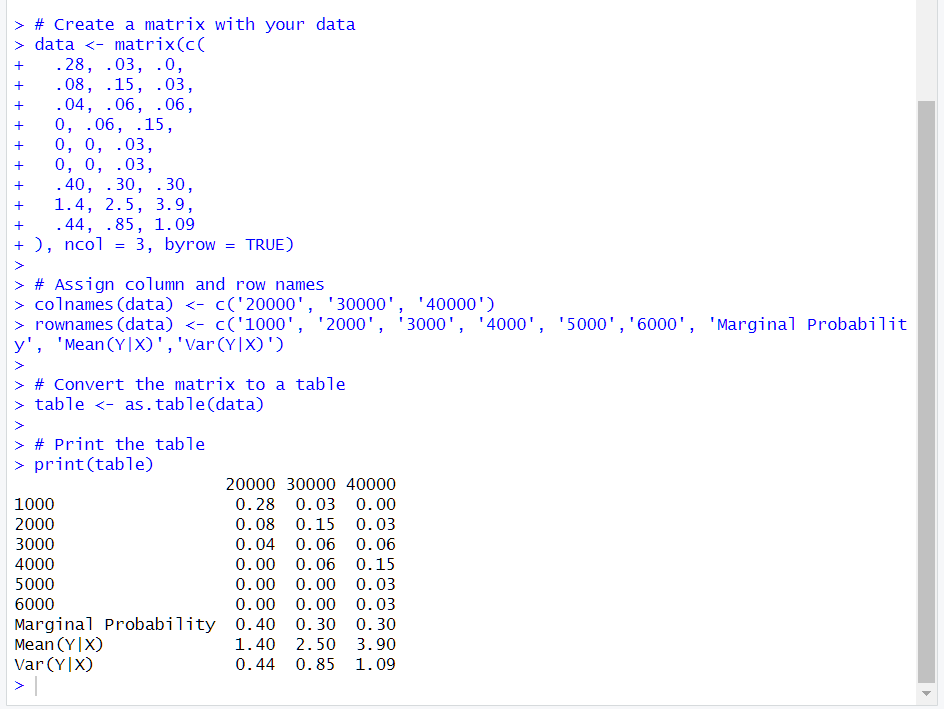
\includegraphics[width=1\linewidth]{imagesfolder/image24.png}
\end{figure}

\begin{spverbatim}

# This line loads the xtable library. The xtable library is an R package that provides an easy way to export tables from R to LaTeX or HTML.
library(xtable)

# Here, the xtable() function of the xtable library is used to convert the R table into a LaTeX table. The result is stored in the latex_code variable.
latex_code <- xtable(table)

# This line prints the LaTeX table to the console. The type="latex" argument specifies that the table should be printed as LaTeX code.
print(latex_code, type = "latex")
\end{spverbatim}
The result of these first lines above is this in the Rstudio:
\begin{figure}[H]
    \centering
    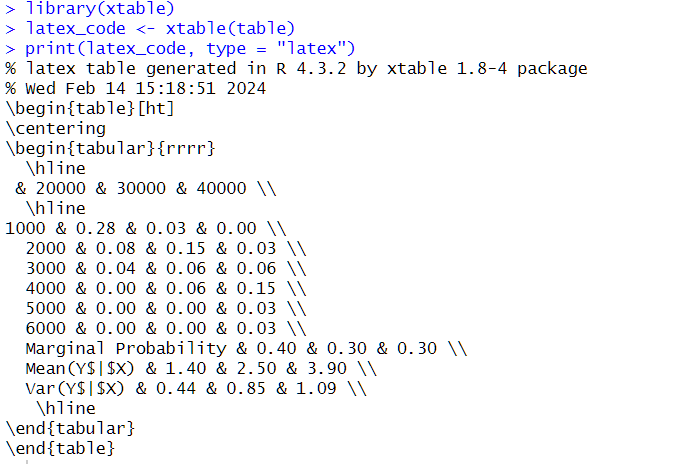
\includegraphics[width=1\linewidth]{imagesfolder/image25.png}
\end{figure}
It would be possible to just paste the text into LaTeX and the table would appear, as in the following image:
\begin{figure}[H]
    \centering
    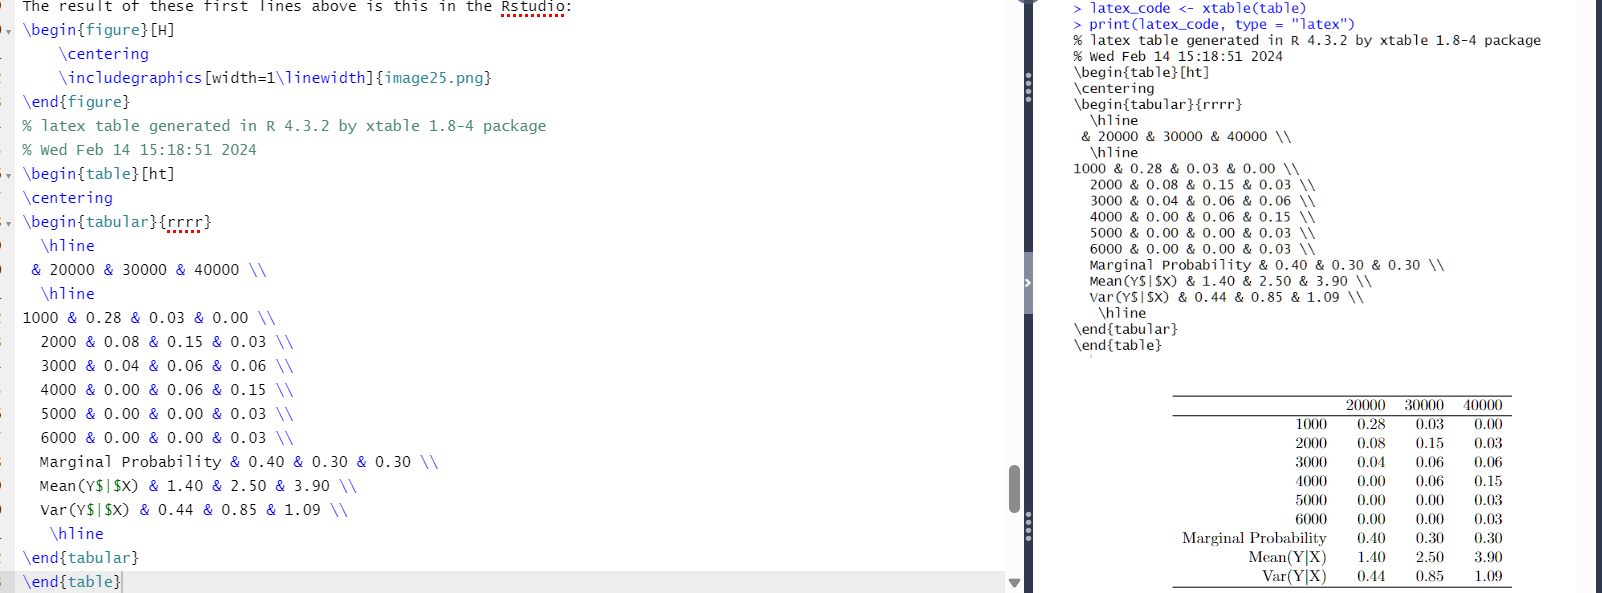
\includegraphics[width=1\linewidth]{imagesfolder/image26.png}
\end{figure}

\begin{spverbatim}
#The sink() function redirects the R console output to a file. In this case, the output will be redirected to the table33.tex file. If the file does not exist, it will be created
sink("table33.tex")

#This line prints the LaTeX table again, but this time the output will be written to the table33.tex file because the sink() function was called previously.
print(latex_code, type = "latex")

#Finally, this line closes the connection to the table33.tex file. This means that the R console output will be redirected back to the console. It is important to always close the connection to the file after you have finished writing to it to avoid problems.
sink()
\end{spverbatim}
The result of these first lines above is this in the Rstudio:
\begin{figure}[H]
    \centering
    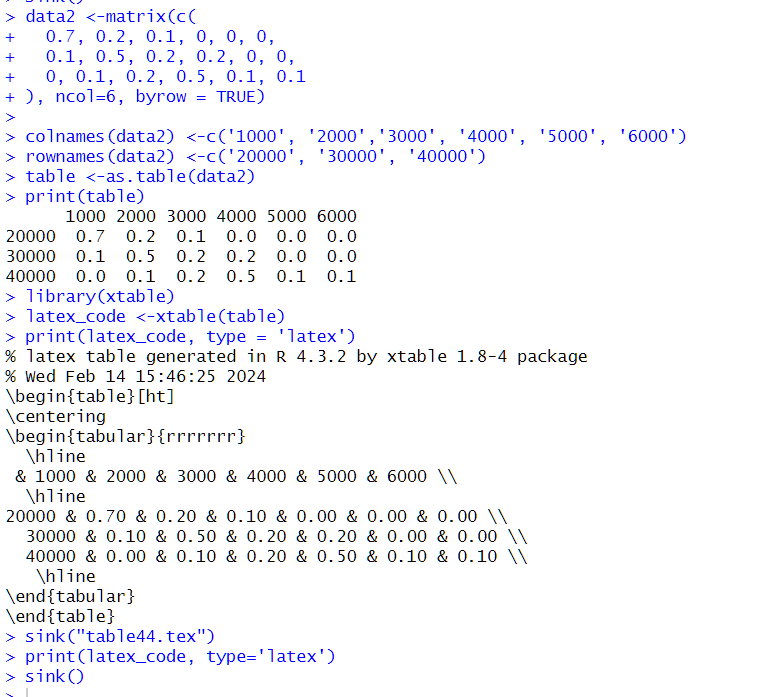
\includegraphics[width=1\linewidth]{imagesfolder/image27.png}
\end{figure}
\begin{figure}[H]
    \centering
    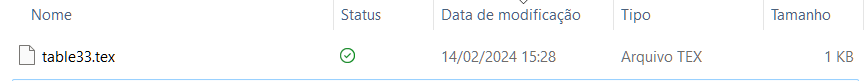
\includegraphics[width=1\linewidth]{imagesfolder/image28.png}
\end{figure}

\begin{spverbatim}

#This line creates a matrix called data2 with 6 columns. Numbers are entered into the matrix row by row (byrow = TRUE).
data2 <-matrix(c(
  0.7, 0.2, 0.1, 0, 0, 0,
  0.1, 0.5, 0.2, 0.2, 0, 0, 
  0, 0.1, 0.2, 0.5, 0.1, 0.1
), ncol=6, byrow = TRUE)

# These two lines assign names to the columns and rows of the data2 matrix, respectively
colnames(data2) <-c('1000', '2000','3000', '4000', '5000', '6000')
rownames(data2) <-c('20000', '30000', '40000')

# This line converts the data2 array into a table. The as.table() function is used for this conversion.
table <-as.table(data2)

# This line prints the table to the console. The print() function is used for this printing.
print(table)

#This line loads the xtable library. The xtable library is an R package that provides an easy way to export tables from R to LaTeX or HTML.
library(xtable)

# This line uses the xtable() function from the xtable library to convert the R table into a LaTeX table. The result is stored in the latex_code variable.
latex_code <-xtable(table)

# This line prints the LaTeX table to the console. The print() function is used for this printing. The type = 'latex' argument specifies that the table should be printed as LaTeX code.
print(latex_code, type = 'latex')

# This line redirects the R console output to a file called table44.tex. The sink() function is used for this redirection. If the file does not exist, it will be created.
sink("table44.tex")

# This line prints the LaTeX table again. However, this time the output will be written to the table44.tex file because the sink() function was called previously.
print(latex_code, type='latex')

# This line closes the connection with the table44.tex file. This means that the R console output will be redirected back to the console. It is important to always close the connection to the file after you have finished writing to it to avoid problems.
sink()
\end{spverbatim}
The result of these first lines above is this in the Rstudio:
\begin{figure}[H]
    \centering
    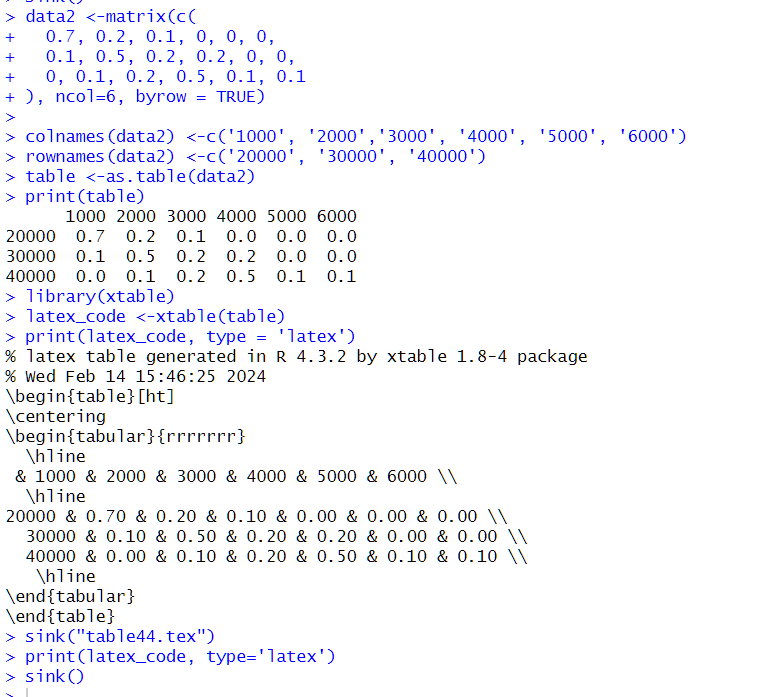
\includegraphics[width=1\linewidth]{imagesfolder/image27.png}
\end{figure}
\begin{figure}[H]
    \centering
    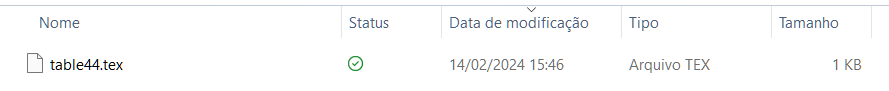
\includegraphics[width=1\linewidth]{imagesfolder/image29.png}
\end{figure}

\end{document}



